\chapter{Background}
\label{c:Background}

\section{Program Comprehension}

\section{Static vs. Dynamic Analysis}

\section{Object Interaction Modeling}
\subsection{UML Object Diagrams}
\subsection{UML Sequence Diagrams}

\begin{figure}
	\centering
	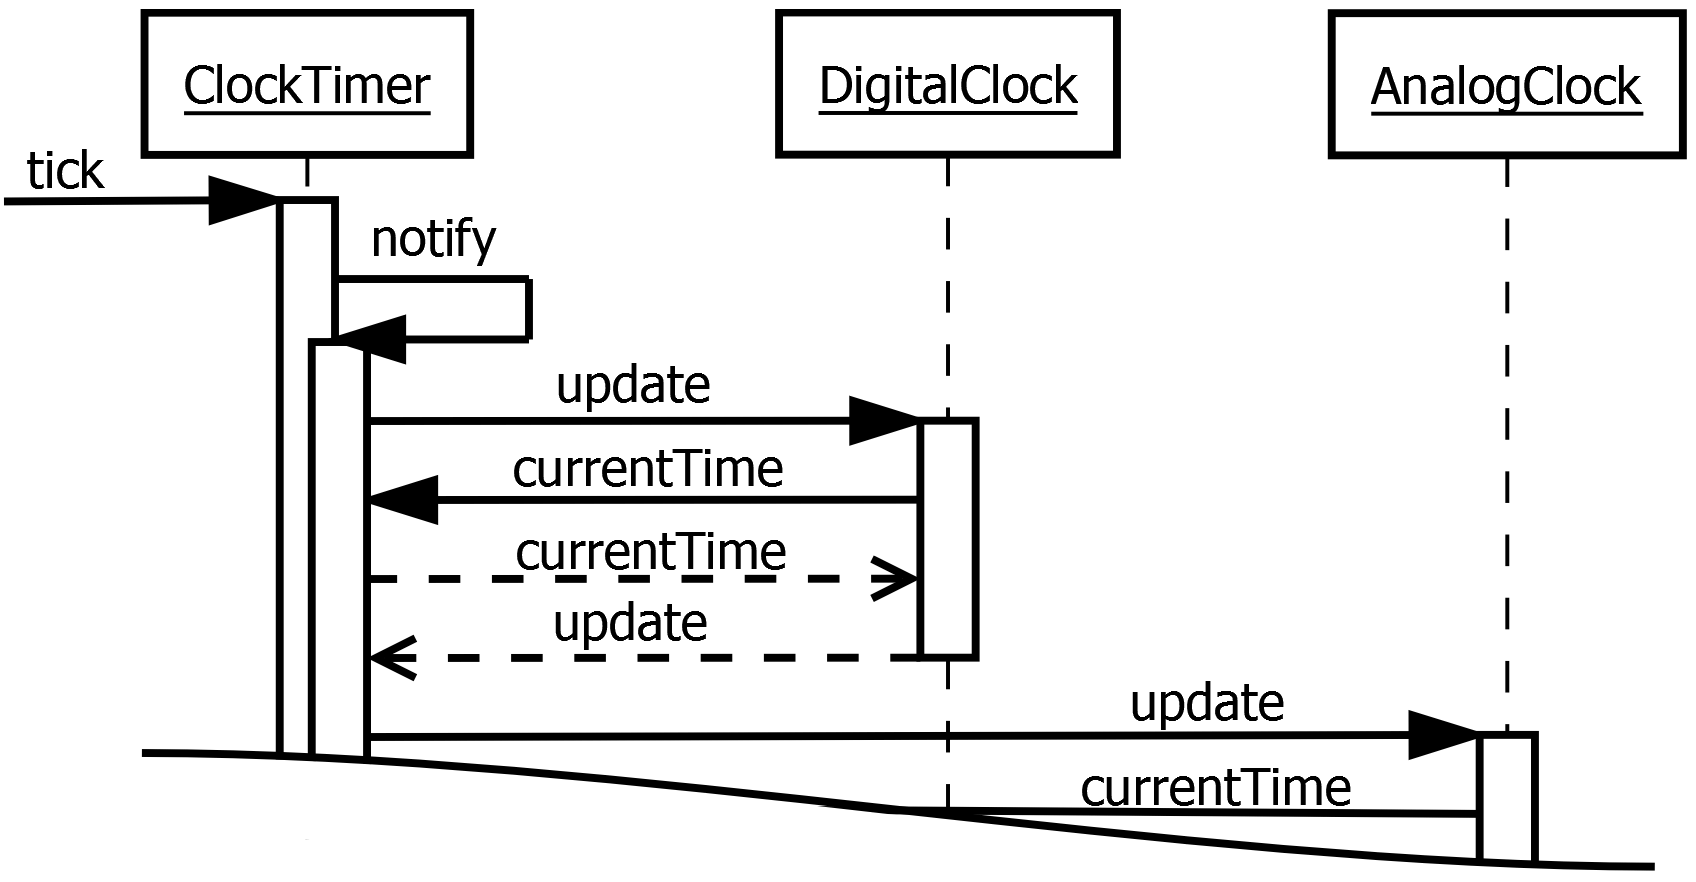
\includegraphics[width=0.8\textwidth]{../images/02-Sequence}
	\caption[TOC Caption]{UML Sequence Diagram}
	\label{fig:ModelingSequence}
\end{figure}


\subsection{UML Collaboration Diagrams}

\begin{smalltalk}[float=htbp,caption=Smalltalk Sample]
newRandomIdInRange: maxVal
	"This is just a sample of smalltalk code"
	
	| pick |
	self objectIds size >= maxVal ifTrue: [self error: 'Woop'].
	
	pick := maxVal atRandom.
	[self objectIds values includes: pick] 
		whileTrue: [pick := pick atRandom].
	^  pick
\end{smalltalk}

\section{Challenges}